\documentclass{article}% [Determines font size] { }Determines type of document (article/beamer/book/etc.)

\usepackage[rightcaption]{sidecap}% Package to produce custom caption positions.
\usepackage{graphicx}% Required package to compile figures.
\usepackage{blindtext}

\begin{document}% Required to produce a compiled LaTeX document. 

\blindtext

\begin{SCfigure}[.25][h]% The SCfigure environment has a few parameter controls: the first box controls the relative size of the caption box in the figure environment. 
        \caption{Complete figure format}% In SCfigure, where the \caption command is place doesn't affect the placement of the title within the figure.
        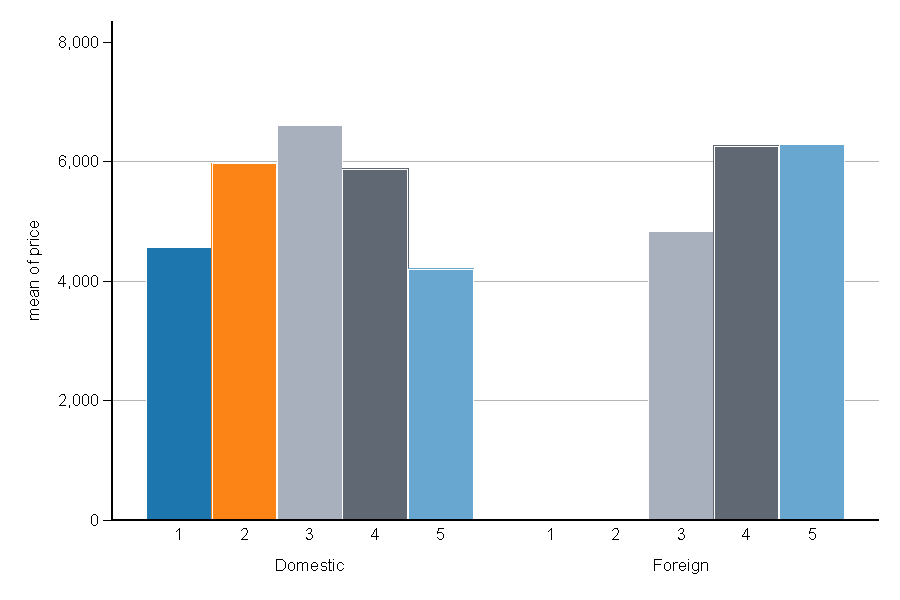
\includegraphics[width=1\textwidth]{figure1.pdf}% [ ] used to customize the size of the figure displayed in document. 
        \label{fig:caption_side}%Use a ":" to create a category of labels on the left side, and the right side is the label of this specific figure.
\end{SCfigure}

\blindtext[4]

\newpage

\end{document}